\documentclass{report}

\usepackage{tikz}
\usepackage{graphicx}
\usepackage{amsmath}
\usepackage{palatino}
\usepackage{siunitx}
\usepackage{hyperref}
\usepackage{listings}

% tables
\usepackage{booktabs}
\usepackage{tabularx}

% begin tikz
\usepackage{tikz}
\usetikzlibrary{graphs,graphdrawing,matrix,decorations.pathreplacing}
\usegdlibrary{layered}
% end tikz

% biblio
\usepackage[style=authoryear]{biblatex}
\addbibresource{references.bib}

\newcommand{\totd}[2]{\frac{D #1}{D #2}}
\newcommand{\pd}[2]{\frac{\partial #1}{\partial #2}}
\newcommand{\bu}{\mathbf{u}}
\newcommand{\ub}{\bar{u}}
\newcommand{\tavg}[1]{\langle #1 \rangle}
\newcommand{\bavg}[1]{\langle \overline{#1} \rangle}
\newcommand{\brunt}{Brunt-V\"ais\"al\"a\ }
%%% Local Variables:
%%% mode: latex
%%% TeX-master: "report"
%%% End:


\title{Moist Convection ML}
\author{Noah D. Brenowitz}
\date{\today}

\begin{document}
\maketitle
\tableofcontents

\chapter*{Notation and Physical Constants}
\label{ch:notation}
\begin{table}
  \centering
  \begin{tabularx}{\textwidth}{lX}
    \toprule
    Symbol & Description\\
    \toprule
    $n$ & number of samples \\
    $m$ &  number of features\\
    $X$ & $s \times m$ data matrix of predictors\\
    $Y$ & $s \times \cdot $ data matrix of predictands\\
    \bottomrule
  \end{tabularx}
  
  \caption{List of common notations}
  \label{tab:constants}
\end{table}

\begin{table}
  \centering
  \begin{tabularx}{\textwidth}{lcX}
    \toprule
    Variable & Value & Description\\
    \toprule
    $c_p$ & \SI{1004}{J/K/kg} & Heat capacity of air\\
    $L_v$ & \SI{2.5e6}{J/kg} & Latent heat of vaporization\\
    \bottomrule
  \end{tabularx}
  
  \caption{List of physical constants}
  \label{tab:constants}
\end{table}
\chapter{Introduction}

\chapter{Training Data}

\section{System for Atmospheric Modeling}
\label{sec:sam}

The System for Atmospheric Modeling (SAM) uses a different set of prognostic
equations \autocite{Khairoutdinov2003}. These are given by

\begin{subequations}
  \label{eq:sam}
  \begin{align}
    &\totd{\bu}{t} + ( f  + \beta y) \mathbf{k}\times \bu = - \nabla \phi \\
    &\totd{w}{t} = -\nabla \phi + g B \label{eq:w-full}\\
    &\totd{h_L}{t}  = Q_{rad}  - \frac{1}{\rho_0} \pd{}{z} \left( L_c P_r + L_s P_s + L_s P_g \right)\\
    &\totd{q_T}{t} = -  \dot{q}_p^{\text{micro}} \label{eq:sam-qT}\\
    &\totd{q_p}{t} = \frac{1}{\rho_0} \pd{}{z} \left(  P_r +  P_s + P_g \right) + \dot{q}_p^{\text{micro}}\\
    &\nabla \cdot \bu + \frac{1}{\rho_0} \pd{\rho_0 w}{z}  = 0.
  \end{align}
\end{subequations}
I have neglected the sub-grid-scale flux terms in the formulation above since
they are not relevant to the problem considered in this report. The temperature
and humidity variables introduced in the previous section have been replaced
here by
\begin{description}
\item[Liquid/ice water static energy] $h_L = c_p T +gz - L_c (q_c + q_r) - L_s
  (q_i + q_s + q_g)$,
\item[Total nonprecipitating water] $q_T = q_v + q_c + q_i$, and
\item[Total precipitating water] $q_p = q_r + q_s + q_g$.
\end{description}
Note that $h_L$ is only an appropriate variable when hydrostatic balance or
anelastic equations are satisfied. Otherwise, potential temperature should be
used. There are a number of diagnostic equations which can be solved to
determine the temperature, and all the mixing ratios for the different species
of precipitating and non-precipitating water. Perhaps most importantly, the
water vapor is assumed to be at or below an approximate saturation value so that
\[q_v = \min(q_T, q_{sat}(p_0, T)),\]
where
\[ q_{sat} = q_{sw} (1-\omega_i) + \omega_i q_{si}\]
is a convex combination of the saturation mixing ratios of vapor with respect to
ice and liquid water. 

A consequence of this diagnostic relation is that the latent
heating term due to condensation is not explicitly calculated. Instead, SAM
models the microphysical processes which govern the conversion from condensate
($\text{cloud water} + \text{cloud ice}$) to precipitation ($\text{rain} +
\text{snow} + \text{grauppel}$). These processes are given by
\[
  \dot{q}_p^{\text{micro}} = \text{accretion} - \text{evaporation} + \text{autoconversion}.
\]
A nice paper by \textcite{hernandez-duenas_minimal_2013} contains a more thorough
discussion of a similar set of microphysical equations, which can be helpful for
gaining intuition. Additional details about the diagnostic relations linking the
water species and the prognostic variables $q_T$, $h_L$, and $q_p$ are available
in Appendix \ref{sec:diag-q} and in the original SAM paper by \textcite{Khairoutdinov2003}.

This formulation is convenient for numerical modeling purposes, but
moist-convective processes are often understood as a coupling between dry
dynamics and moist variables because the bouyancy is related primarily to
temperature, rather than moist static energy.
For instance, the circulation due to the monsoons and MJO can be understood
roughly as the response to a imposed heating pattern \autocite{Gill1980}, and
the multiscale theories of Biello and Majda rely upon asympotic analysis of the
latent heating.

\section{Near-global Model Configuration}
\label{sec:model-config}

We configure the model in the same way as \textcite{Bretherton2015}. 

The size of the domain is (5120, 2560) grid points with a grid size of
\SI{4}{\km}, which in physical units is \SI{20480}{\km} by \SI{12800}{\km}.
We define the central 2560 kilometers in the y-direction as the tropics. 
This is 16 coarse grained grid boxes out of total of 64, which is [24, 40) in
0-indexed notation.

\begin{figure}[ht]
  \centering
  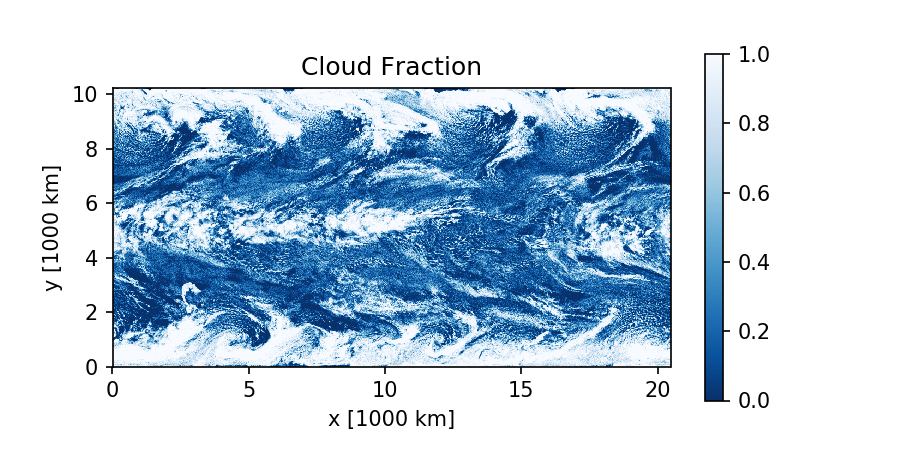
\includegraphics{images/cld.png}
  \caption{\label{fig:cld}Snapshot of the cloud cover fraction field from the NGAqua simulation.}
\end{figure}

% \begin{tikzpicture}[scale=.5]
%   \draw (0,0) rectangle (20.480, 12.800);
%   \draw[step=.160] (0,0) grid (20.480, 12.800);
% \end{tikzpicture}


\section{Data Availability}

The coarse-grained NGAqua data is available on the olympus file server in the UW Atmospheric Sciences department as well as in a google cloud storage bucket:
\verb|nbren12-largedata/data/id/726a6fd3430d51d5a2af277fb1ace0c464b1dc48|

\section{Model Outputs}

The model outputs a collection of three dimensional and two dimensional fields
at a sampling interval of three hours. 
Because the model uses an Arakawa C-Grid, some of the variables are staggered
while others are centered. 
Figure \ref{fig:arakawa-c-grid} provides an illustration of this.

\begin{figure}
  \centering

  \begin{tikzpicture}[scale=2]


    \draw (-1, 0) -- (3,0);
    \draw (0, -1) -- (0,3);
    \draw (2, -1) -- (2,3);
    \draw (-1, 2) -- (3,2);
    
    \node at (1,1) {$q_v$, $q_p$, $q_n$, $\phi$, $s_l$};
    \node[fill=white] at (1,0) {$u_{i}$};
    \node[fill=white] at (1,2) {$u_{i+1}$};
    \node[fill=white] at (2,1) {$v_{i+1}$};
    \node[fill=white] at (0,1) {$v_{i}$};
  \end{tikzpicture}

  \caption{Arakawa C-Grid. 
    The velocities are represented on the faces, while the scalar quantities are
    cell-centered. 
    This plot only shows the horizontal grid, but the vertical velocity $w$ is
    staggered in the vertical direction.}
  \label{fig:arakawa-c-grid}
\end{figure}


\section{Coarse-graining and Destaggering}
\label{sec:post-processing}

The main post processing steps are

\begin{enumerate}
\item Coarse-graining, and 
\item computing the apparent heat and moisture source due to convection.
\end{enumerate}

The coarse graining procedure is relatively straightforward. 
SAM outputs the data on a grid with a \SI{4}{\km} resolution. 
We can describe this coarse-graining mathematically. 
Let $f(x,y,z,t)$ be some three dimensional field outputed by the atmospheric
model. 
Then, divide the domain into coarse grained grid boxes $C_{i,j}$ which represent the
typical GCM grid box. These grid boxes are defined by

\[
  C_{i,j} = \{(x,y):   j \Delta x \leq x < (j+1) \Delta x
  \quad \cap\quad j \Delta y \leq y < (j+1) \Delta y \},
\]
where $\Delta x$ and $\Delta y$ are the size of the GCM grid box (e.g.
\SI{160}{\km}). Averaging over these grid boxes gives the coarse-grained field
\[
  \overline{f}_{i,j} = \int_{C_{ij}} f dA.
\]

\begin{figure}
  \centering
  \begin{tikzpicture}
    \draw (0,0) rectangle (6,6);
    \draw[step=1.5mm] (0,0) grid (6,6);
    \draw[decorate,decoration={brace,amplitude=10pt,mirror,raise=4pt}] (0,0) -- (6,0);
    \node at (3,-.7cm) {$\Delta x = \SI{160}{\km}$};
  \end{tikzpicture}
  \caption{Coarse-graining procedure. The coarse-grained grid boxes have a
    length of \SI{160}{km} and contains $40^2$ fine scale grid boxes.}
  \label{fig:coarse-grain}
\end{figure}

Figure \ref{fig:preprocess} contains a flow chart describing the preprocessing pipeline.

\begin{figure}
  \centering
  \begin{tikzpicture}[ every node/.style={draw} ]
    \graph[layered layout]{

      Input data -> Destagger $u$ and $v$ -> a/ Coarse grain all variables;
      Input data -> a; a -> w/Destagger coarse grained $\overline{w}$; {a, w} ->
      Reshape data and fit models!

    };
  \end{tikzpicture}
  
  \caption{Preprocessing pipeline flowchart}
  \label{fig:preprocess}
\end{figure}
\section{Apparent Heating and Moistening}
\label{sec:q1q2}

In SAM, the conserved variables are the liquid-ice static energy and the total non-precipitating water. The liquid static energy is given in temperature units by 
\[ s_l = T + \frac{g}{c_p} z - L_c(q_n + q_p),\]
where $q_n$ is the total cloud condensate, $q_p$ is precipitation, and $L_c$ is the latent heat of condensation. This definition is an approximation which neglects the presence of the frozen phase of water. The total water non-precipitating water is just given by 
$q_t = q_v + q_n.$

Then, for our purposes, the apparent heat source is given by
\[Q_1 = \partial_t {s_l} + \mathbf{v}\cdot \nabla s_l, \]
and the apparent drying is given by
\[Q_2 = - \frac{L_c}{c_p} \left[\partial_t {q_t} + \mathbf{v} \cdot \nabla q_t\right].\]
The factor $-\frac{L_c}{c_p}$ is used to ensure that this quantity also has units K/day. Comparing to the original prognostic equations for SAM shows that $Q_1$ contains the source term  $Q_r$ to the temperature equation which represents radiative transfer, which is usually a cooling tendency. For the purposes of cumulus parametrization, it might be possible to assume this is known from other sources (e.g. a radiative transfer code such as RRTMG). Therefore, we will also define the convective component of the apparent heating as $Q_{1c} = Q_1 - Q_r$. 

All the differential operators in these two expression represent a finite
differencing taken on the coarse grid, and we will use centered differences to
compute these. Specifically, the formulas for the advection terms are given
by
\renewcommand{\bf}{\bar{f}_{i,j}}

% \[(A_f)_{i,j} = \left( \bar{f}_{i+1,j,k} - \bar{f}_{i-1,j,k} \right) \frac{\bar{u}_{i,j,k}}{2 \Delta x}
%               + \left( \bar{f}_{i,j+1,k} - \bar{f}_{i,j-1,k} \right) \frac{\bar{v}_{i,j,k}}{2 \Delta y}
%               + \left(  \bar{f}_{i,j,k+1} - \bar{f}_{i,j,k-1} \right) \frac{\bar{v}_{i,j,k}}{z_{k+1} - z_{k-1}}
%             \]

\begin{align}
  (A_f)_{i,j,k} = &\left( \bar{f}_{i+1,j,k} - \bar{f}_{i-1,j,k} \right) \frac{\bar{u}_{i,j,k}}{2 \Delta x}\\
              +&\left( \bar{f}_{i,j+1,k} - \bar{f}_{i,j-1,k} \right) \frac{\bar{v}_{i,j,k}}{2 \Delta y}\nonumber\\
              +& \left(  \bar{f}_{i,j,k+1} - \bar{f}_{i,j,k-1} \right) \frac{\bar{w}_{i,j,k}}{z_{k+1} - z_{k-1}}.\nonumber
\end{align}
We have taken advantage of the constant horizontal grid spacing and the
collocation of all the coarse grained variables.

The numerical estimates of $Q_1$ and $Q_2$ depend on these simple expressions.
The apparent heating is given by
\begin{equation}
  \label{eq:q1-num}
  Q_1^{n+1/2} = \frac{\bar{s_l}^{n+1} - \bar{s_l}^{n} }{\Delta t}
            + \frac{1}{2} \left( A^{n+1}_{s_l}  + A^{n}_{s_l} \right).
\end{equation}
where the spatial index $i,j,k$ has been dropped. Similarly, the apparent
drying is given by
\begin{equation}
  \label{eq:q2-num}
  -\frac{c_p}{L_v} Q_2^{n+1/2} = \frac{\bar{q_T}^{n+1} - \bar{q_T}^{n} }{\Delta t}
            + \frac{1}{2} \left( A^{n+1}_{q_T}  + A^{n}_{q_T} \right).
\end{equation}
The factor $\frac{c_p}{L_v}$ ensures that $Q_2$ has units of temperature over
time, just like $Q_1$. These and other important physical quantities are
described in \autoref{tab:constants}.

\section{TODO Reshaping data}

Most machine learning algorithms require two dimensional matrices as inputs, so
we will have to reshape the training data to achieve this. Because the
time-scale of deep atmopsheric convection is so fast, the inputs for the
convection scheme should be non-local in the vertical direction.

\chapter{Methods}

\section{Machine Learning for dynamical systems}

The ultimate goal of this work is to estimate or simulate the unknown source
terms. Essentially we need an effective way to draw samples
from
\[ \rho(x_{t+\Delta t}, t + \Delta t |x_{[s < t]}).\] There are two clear problems here. 
First, this probability distribution depends on the whole time course of
$x$ leading up to time $t$. 
Ideally we want to create a Markov description of the data, a task which is
known as \emph{embedding}. 
Supposing $z_t$ is a suitable embedding of $x_t$---Takens' delay embedding is a natural choice---the conditional pdf becomes
\[\rho(z_{t+\Delta t}, t+ \Delta t| z_t, t),\]
and we must characterize this conditional density.
We also might prefer to use the infinitesmimal generator
\[L_z = \lim_{\Delta t \rightarrow 0} \frac{\rho(z_{t+\Delta t}, t+ \Delta t| z_t,
    t) - \delta(z_{t+\Delta t} - z_t) }{\Delta t}.\]

There are also a series of functions $f_i$ which we trust capture some aspect of
the dynamics. 
For example, we should trust the dynamical core, turbulence, and radiation
schemes, and not attempt to \emph{learn} a GCM from scratch.
But the functions $f_i$ are not specified in the pdf at all, and we might not
even know them with perfect accuracy. We can include them in the statistical
model as follows
\[\rho(z_{t+\Delta t}, t+ \Delta t| z_t, y_i, t) p(y_i|z_t, t) \]
where $y_i = f_i(z_t) + \epsilon_i$.




\section{Maximum Covariance Analysis}
\label{sec:mca}

\begin{figure}
  \centering
  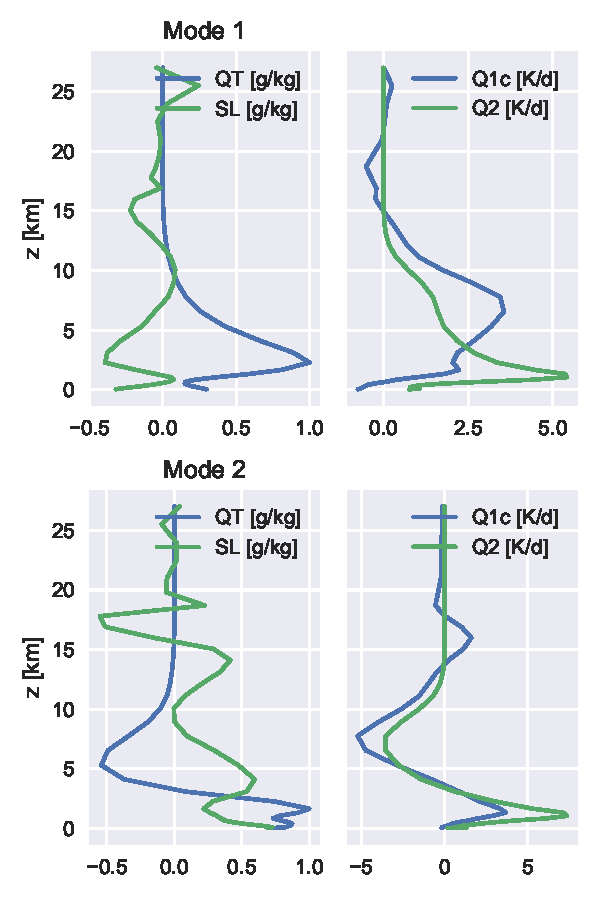
\includegraphics[height=5in]{images/mca_modes.pdf}
  \caption{Loadings for first two MCA modes.}
  \label{fig:mca-loadings}
\end{figure}
\begin{figure}
  \centering
  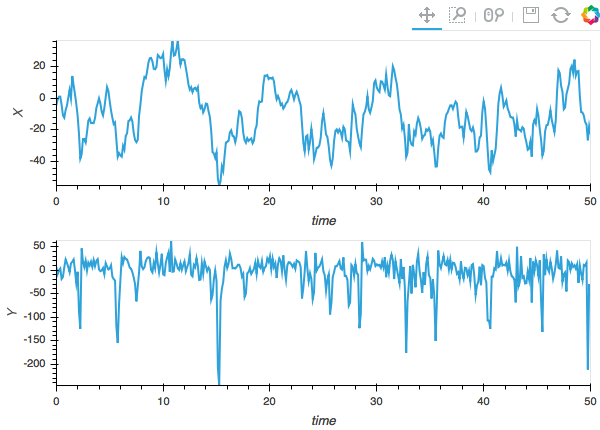
\includegraphics[width=\textwidth]{images/mca_ts.png}
  \caption{Time series of first MCA mode scores for a location at the equator. 
    Input scores (top) and output scores (bottom).}
  \label{fig:mca-ts}
\end{figure}
\printbibliography

\appendix

\chapter{Source code}
\label{sec:source}

% \lstinputlisting[language=python]{../lib/linear_regression.py}

\end{document}

% Local Variables:
% TeX-master: t
% End:
